\chapter{Introduction}
\label{:intro}

Range searching is one of the most common types of problems which arise in everyday computer use. 
With a range search, we are given a set of objects and asked to identify those which satisfy some bounded criteria. 
Range searches can take many different forms: searching for email received between two dates, looking for restaurants near your present location, or identifying what a video game player should see on their screen in any one frame; these are all examples of range searches.

In computational geometry, range searching takes on a more abstract quality. 
Typically we are given an environment containing a set of geometric objects such as points, lines, circles, or boxes. 
A query is itself another well-defined geometric object, and our goal is to identify all elements of the environment contained within the query region.  
When addressing a range searching problem, we want to develop a method for preprocessing the input environment so that we can answer any query as efficiently as possible.
Given how common and flexible range searching is to such a wide range of practical computer science, it is not surprising to  find that a great deal of research has been expended in this area.  

In this thesis, we address the notion of \emph{Partial Enclosure Range Searching (\PERS{})}, which, to the best of our knowledge, has not been explored previously. 
In this setting, our goal is to identify, for a given query region, all objects which satisfy the \emph{Partial Enclosure Property}, which specifies that an object must intersect a query region by at least some fixed proportion of the object's own size (e.g., length, area, volume) in order to be selected.

This chapter is organized as follows.
Section~\ref{:intro:motivation} begins by describing our motivation for this problem. 
In Section~\ref{:intro:problems} we describe the specific variations of the \PERS{} problem that we will address in this thesis. 
In Section~\ref{:intro:related}, we discuss related problem domains, and contrast them to our own.
Section~\ref{:intro:contributions} outlines the contributions made by this thesis.
We conclude the introduction by outlining the organization of the remainder of the thesis in Section~\ref{:intro:organization}.


%------------------------------------------------------------------------------
%------------------------------------------------------------------------------
\section{Motivation}
\label{:intro:motivation}

This problem was inspired by the author's use of Microsoft OneNote. 
Using a digital pen, OneNote can be used much like a paper notebook, allowing the user to add handwriting, diagrams, equations, and any other such thing to a page.
Unlike a paper notebook, OneNote also allows the user to select previously drawn objects in order to translate, scale, copy and otherwise manipulate them.
Figure~\ref{fig:intro:onenote} shows some handwritten notes, and a diagram which has been partially selected.

\begin{figure}
\begin{center}
  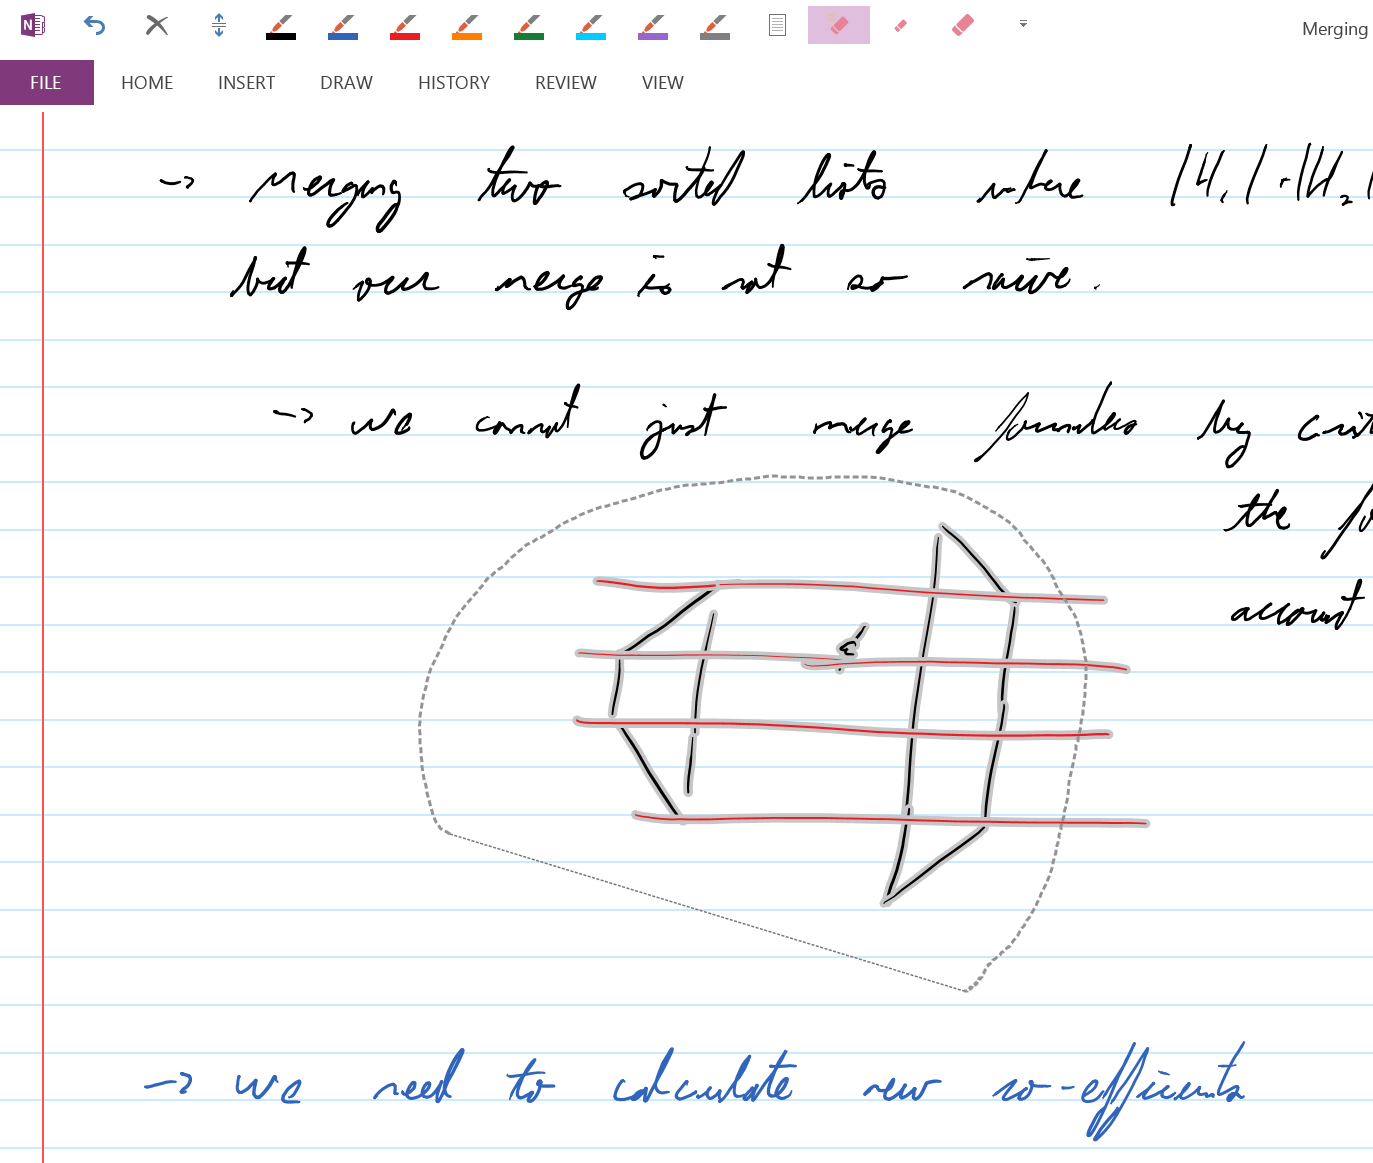
\includegraphics[width=0.50\textwidth]{figures/fig_onenote}
  \caption[An example of practical partial enclosure range searching]{An example of practical partial enclosure range searching in Microsoft OneNote. The line segments in the middle are selected even though they are not entirely enclosed.}
  \label{fig:intro:onenote}
\end{center}
\end{figure}

Looking carefully at the figure, we can see that even though the horizontal line segments of the diagram have not been entirely enclosed by the selection tool, they nevertheless appear as part of the set of selected items.
This behaviour of selecting partially enclosed objects is described in a patent filed by Microsoft Corporation\cite{lassoselect}. 
From the patent:

\begin{quote}
[T]here is a need for a selection tool that will allow a user to conveniently select one or more graphical objects in their entirety, without requiring an inconvenient amount of precision from the user.
\end{quote}

\noindent With the rising popularity of touch and pen-enabled devices, this need is likely to increase.  
As we can see from the figure, OneNote already includes an implementation of a partial selection tool like the one described by the patent. 
Although the details of the implementation are proprietary, it becomes apparent while using the software that it suffers from poor performance as more items are selected.
It is from this observation that the work in this thesis was inspired.  
Although the problems that we will examine take place in simpler settings than the patent describes, we will nevertheless develop an understanding of where the major challenges of this problem domain are found, as well as some techniques for addressing them.


%------------------------------------------------------------------------------
%------------------------------------------------------------------------------
\section{Problem Statements}
\label{:intro:problems}

This thesis proposes algorithms for several different partial enclosure range search settings.  Each problem addresses a different type of geometric object to be queried, or a different type of query region.

\paragraph{Line Segments and Query Rectangles.} Line segments and rectangles are one of the simplest settings in which we can perform partial enclosure range searches. 
Given an axis-parallel query rectangle, we address methods which consider only axis-parallel segments, or which consider arbitrarily-oriented ones.

\paragraph{Line Segments and Query Slabs.} Relaxing the axis-parallel query regions of the preceding problem, we consider an arbitrarily-oriented slab.
As the query slab can have any orientation, intersections with a horizontal segment will involve both the height of the segment and the slope of the slab.  
We also consider a query defined as the intersection of two slabs.

\paragraph{Convex Polygons and Query Rectangles.} Moving away from line segments, we consider problems of partial enclosure with respect to area. 
Starting with convex polygons, we address methods for calculating the area enclosed by a rectangle. 
 
\paragraph{Monotone Polygons and Query Rectangles.} This more complex shape does not generally decompose into big convex regions, so a different method of preprocessing will be needed.
We consider methods for calculating the area of the polygon to one side of a query line. 
With such a method in hand, determining the area of a rectangle is a matter of executing several queries and combining their results.

%------------------------------------------------------------------------------
%------------------------------------------------------------------------------
\section{Related Work}
\label{:intro:related}

We contrast our problem from traditional range searching, which looks for objects which are entirely within a query region, and from intersection searching, which looks for any objects which have even a minimal intersection with a query region.

\paragraph{Range Searching.} 
XXX TODO

Should explain why this is easier than our problem

\paragraph{Intersection Searching.} 
XXX TODO

Should explain why this is easier than our problem

This is either looking at objects that have \emph{any} intersection at all, or which are entirely intersected in a geometric sense; that is $o \cap Q = o$.  Whereas range searching is a bit more abstract.


%------------------------------------------------------------------------------
%------------------------------------------------------------------------------
\section{Summary of Contributions}
\label{:intro:contributions}

In this thesis, we develop contributions to several variations of the \PERS{} problem, along with some noteworthy ancillary methods. 
Table~\ref{tab:contributions} gives a broad overview of the data structures we develop. 
The table uses `AP' for ``Axis-Parallel'', `AO' for ``Arbitrary Orientation'', and `P' for ``Polygon'', and omits ``Big Oh'' for clarity.

\begin{table}[t]
\caption{Summary of Contributions}
\label{tab:contributions}
\centering
\begin{tabular}{l l l l l l}
\hline \hline
Object & Query & Theorem & Space & Time & Query \\
\hline
AP Segment & AP Rectangle & Th~\ref{th:ap} & ${n\log^3{n}}$ & ${n\log^3{n}}$ & ${\log^3{n}}$ \\
AO Segment & AP Rectangle & Th~\ref{th:ao} & ${n\log^7{n}}$ & ${n\log^7{n}}$ & ${\sqrt{n}\log^7{n}}$ \\
AP Segment & AO Slab & Th~\ref{th:slabs:one} & ${n\log^2{n}}$ & ${n\log^3{n}}$ & ${\sqrt{n}\log^3{n}}$ \\
AP Segment & 2 AO Slabs & Th~\ref{th:slabs:two} & ${n\log^3{n}}$ & ${n\log^4{n}}$ & ${\sqrt{n}\log^4{n}}$ \\
Convex P & Rectangle & Th~\ref{th:convexp:area} & ${n}$ & ${n}$ & ${\log{n}}$ \\
Convex P & Convex $k$-gon & Cor~\ref{cor:convexp:karea} & ${n}$ & ${n}$ & ${k \log{n}}$ \\
Monotone P & AP Rectangle & Th~\ref{th:monotonep:rect:area} & ${n\log{n}}$ & ${n\log{n}}$ & ${\log{n}}$ \\
Monotone P & AP Rectangle & Th~\ref{th:mono2} & ${n}$ & ${n\log{n}}$ & ${\sqrt{n}}$ \\
Simple P & Horiz Slab & Cor~\ref{cor:monotonep:simplep-area} & ${n}$ & ${n}$ & ${\log{n}}$ \\
\hline
\end{tabular}
\end{table}

In the line segment cases, we develop methods for restating the partial enclosure property as something which can be evaluated as a one or two variable inequality. 
These expressions can then be queried by known structures for orthogonal or half-plane queries. 
We discuss the transformations to appropriate dual-spaces and the design of data structures which can answer the necessary multi-part queries.

In the polygon cases, we primarily develop methods for calculating area within a simple region, e.g., below a query line.
These methods are then repeated and combined to find the area enclosed by the actual query region.
Once the enclosed area is known, determining the partial enclosure property is straight-forward.

%------------------------------------------------------------------------------
%------------------------------------------------------------------------------
\section{Organization of the Thesis}
\label{:intro:organization}

The remainder of this thesis is organized in the following way. 
Chapter~\ref{:prelim} reviews existing data structures and range searching techniques which we utilize in our own contributions.
The next four chapters cover partial enclosure range searching queries on successively more sophisticated geometric objects, with Chapter~\ref{:rectangles} focusing on axis-parallel rectangles, Chapter~\ref{:slabs} on arbitrarily-oriented slabs, Chapter~\ref{:convexp} on convex polygons, and Chapter~\ref{:monotonep} on monotone polygons.
The thesis concludes with Chapter~\ref{:conclusion} which summarizes the contributions and future work presented in earlier chapters.
